\documentclass{article}
\usepackage{graphicx} 
\usepackage{float}
\title{Diving Into the Mysteries of Fractals}
\author{Julie Rehmeyer}
\date{01.07.2018} 
\begin{document}
\maketitle
How long is a country’s border? That’s the seeming	ly simple question mathematician Lewis Fry Richardson asked himself more than 75 years ago.  \vspace{0.4cm}

The thing that puzzled him was that the length of the measuring stick mattered. Let’s use Great Britain as an example: Use a 100-mile ruler, and you get one answer for total coastline. But if you reduce that ruler to a mile, it will fit inside bays the larger ruler missed, and the answer will be far larger. An inch-long ruler will give a still-larger result.  \vspace{0.4cm}

Indeed, Richardson realized, the answer depended entirely on the length of the measuring stick. The shorter it is, the longer the measurement. Taken to its conclusion, the answer was striking: The coastline of Britain is infinite.  \vspace{0.4cm}

He didn’t know it, but Richardson had just stumbled on a previously unrecognized type of geometric object, one that was destined to revolutionize traditional mathematics. He’d found a fractal.
\section{Fractal Fabrication}
\begin{figure}[H]
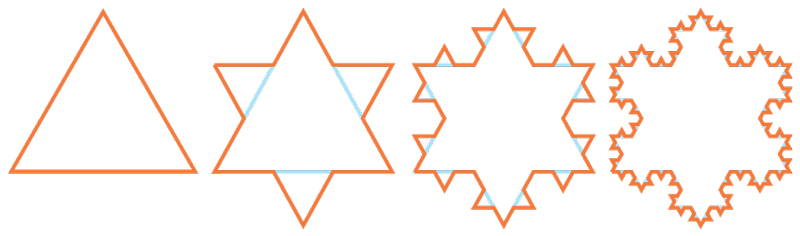
\includegraphics[scale=0.43]{snowflakes.jpg}
\caption{Snowflakes}{Snowflakes form fractals in real life, not just in Koch’s mathematical imagination. Ice crystallizes around a speck of dust in the atmosphere, and the shape of the water molecules results in six-sided symmetry. The precise atmospheric conditions at each moment of creation determine whether the snowflake will form a branch at each point. Alison Mackey/Discover}
\end{figure}
A fractal is like an infinite version of a Russian nesting doll: Zoom in on one, and you get a smaller version, more or less, of what you started with. A coastline is a fractal because at any scale, you’ll find coves and bays — well, at least until you get down to atoms.

In the realm of pure mathematics, though, there are no such practical limitations. Consider, for example, the \begin{quote}"Koch snowflake"\end{quote} (below, in red), named after Swedish mathematician Helge von Koch. Start with an equilateral triangle, and then on each side erase the middle third and replace it with a smaller equilateral triangle. Do it again and again — forever.

What you get has a similar quality to a real-life coastline — and the more steps you complete in constructing it, the longer the perimeter gets. Do it forever, and you’ll end up with an infinitely long border — though all that infinitude still contains a finite area. It’s like a mathematical version of a saying by the 13th-century poet Rumi: \begin{quote}"You are the entire ocean in a drop."\end{quote}
\section{Other Famous Fractal Figures}
\begin{figure}[H]
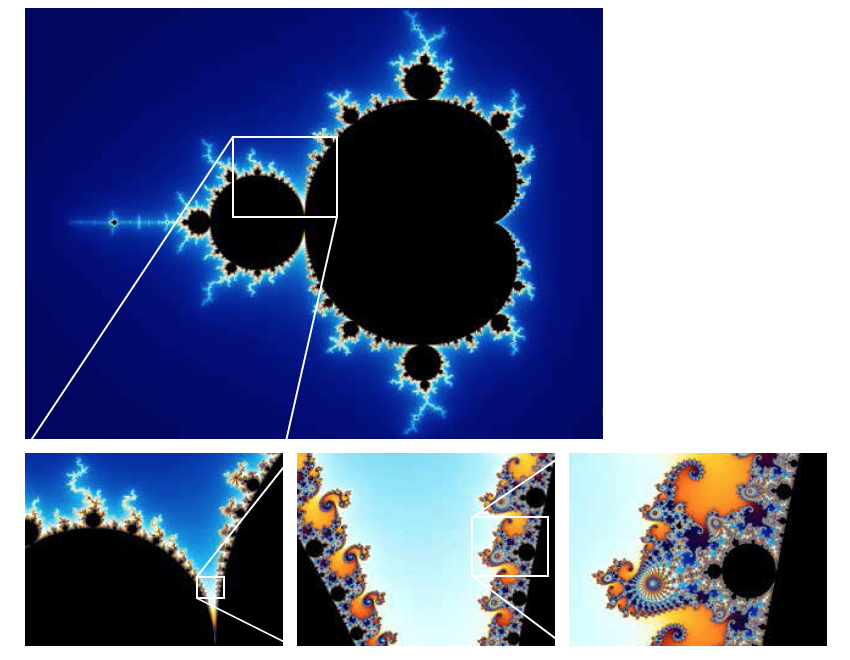
\includegraphics[scale=0.43]{ScreenShot20180605at21515PM.jpg}
\caption{Wolfgang Beyer via Wikimedia}
\end{figure}
\subsection{The Mandelbrot Set }
In 1978, mathematicians Robert W. Brooks and Peter Matelski — in the process of answering a very different mathematical question — defined a new object based on an equation that is, by their standards, quite simple. But the wonders of this object didn’t become clear until March 1, 1980, when mathematician Benoit Mandelbrot programmed a computer to draw it.

He discovered an object unlike any he’d ever seen. At the largest scale, it’s a kind of heart shape with a circular tail. Zoom in, and you’ll find worlds within worlds within worlds, with shapes resembling sea horses, galactic whorls and mandalas. But within each of these fantastical shapes, the original heart-shaped figure also hid. A single equation contained an entire mathematical universe.
\begin{figure}[H]
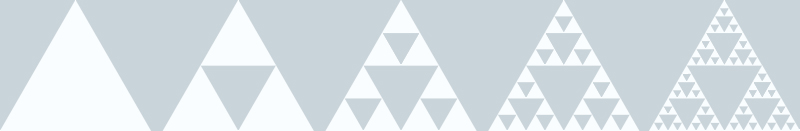
\includegraphics[scale=0.43]{DSC-B0818_Sierpinski.jpg}
\caption{Alison Mackey/Discover}
\end{figure}
\subsection{The Sierpinski Triangle}
Here’s another you can make yourself. Start with an equilateral triangle and divide it into four equal-sized, smaller equilateral triangles, then remove the center one. Repeat that process with the three remaining triangles — forever. You’ll end up with a Sierpinski triangle, named after Polish mathematician Wacław Franciszek Sierpin’ski. Amazingly, its area is zero.
\section{Interdimensional Reality}
Fractals often have the rare property of existing between our ordinary dimensions.

The Koch snowflake, for example, consists of ordinary one-dimensional lines, but with more and more iterations, it appears fuzzy, as if it had breadth. The Sierpinski triangle is built from an ordinary two-dimensional triangle, but with all the area carved out, it doesn’t quite have the heft of two dimensions.

Mandelbrot captured this through the idea of a fractional dimension — hence the name fractal. Essentially, it captures how complex and squiggly a fractal is. Think again of a coastline: As you shrink your measuring stick, the apparent length of a craggy coastline will grow much faster than that of a smooth beach, so it will accordingly have a higher fractal dimension.

The Koch snowflake has a fractal dimension of about 1.26, and the Sierpinski triangle is a bit higher at 1.58. And the boundary of the Mandelbrot set has fractal dimension of 2 — meaning it is as rough a coastline as it could possibly be. It took until 1991 to prove that.
\section{Fractal cities and city fractals}
Is the coast of Britain a real fractal line? In fact, we cannot find any real fractals (based on fractal
geometry) in the real world. This is like that we cannot find circles and triangles (based on Euclidean
geometry) in the real world. All of the fractal images we encounter in books and articles represent
pre-fractals rather than real fractals in mathematical sense. A real fractal has infinite levels, which
can only be revealed in the mathematical world, but a pre-fractal is a limited hierarchy, which can
be found in any textbooks on fractals. We can use the ideas from fractal geometry to research prefractals, including regular pre-fractals and random pre-fractals. The coast of Britain can be regarded
as a pre-fractal curve instead of a real fractal line. However, we can study the coast of Britain using
the ideas from fractals and fractal dimension. Similarly, cities are not true fractals, but proved to be
random pre-fractals because urban form has no characteristic scales. A great number of empirical
studies show that, based on certain scaling range, urban form satisfy three necessary and sufficient
conditions for fractals (Table 1). Urban form follow power laws, which indicates that cities can be treated as pre-fractals. The basic property of a random pre-fractal object is that its scaling range is
limited, and its fractal dimension value is based on the scaling range (see, e.g., Addison, 1997). 

\centering
\begin{table}[h]
\caption{Three necessary and sufficient conditions for fractals}
\begin{tabular}{|l|l|p{4.2cm}|}
\hline
Conditions & Formula & Note \\
\hline
Scaling law & $Tf(x)=f(\lambda x)=\lambda^b f(x)$ & The  relation between scale and the
corresponding measures follow power laws \\
\hline
Fractal dimension & $d_{T} < D < d_{E}$ & The fractal dimension D is greater than the
topological dimension $d_{T}$ and less than the
Euclidean dimension of the embedding space $d_{E}$ \\
\hline
Entropy conservation & $\displaystyle\sum_{i=1}^{N(r)}P_{i}^q r_{i}^{(1-q)D_{q}} = 1$ & Then Renyi entropy values of different fractal
units (fractal subsets) are equal to one another. \\
\hline
\end{tabular}
\small
Note: T-scaling transform; $x$-scale variable; $f(x)$-a function of $x$;$\lambda$-scale factor; $b$-scaling exponent; D-fractal dimension; $d_{T}$-topological dimension; $d_{E}$-Euclidean dimension of embedding space; $q$-order of moment;
$P_{i}$,$r_{i}$-growth probability of the ith fractal set and its linear scale; $D_{q}$-generalized correlation dimension.

\end{table}

\section{Nature's Favorite Patterns}
\begin{figure}[H]
\centering
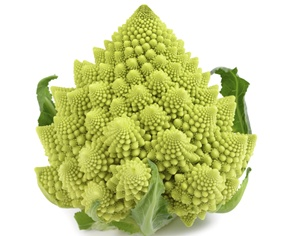
\includegraphics[scale=1]{DSC-B0817_07.jpg}
\caption{Scisettialfio/istock}
\end{figure}
Mandelbrot titled one of the books in which he introduced these ideas The Fractal Geometry of Nature. While Mother Nature doesn’t form patterns that perfectly repeat forever, the way mathematical fractals do, she does create some gorgeous approximations.
\begin{itemize}
\item \textbf{Romanesco} -- related to broccoli, is a particularly striking and beautiful example, with spirals made of spirals made of spirals made of spirals.

\item \textbf{Lightning} -- forms a fractal pattern with its branching branches, which means that it has a fractal dimension — one study approximated it at 1.51. When people are struck by lightning, it can form a lightning-shaped mark as the electricity travels across the skin, damaging blood vessels — which themselves form a branching, fractal-like pattern.
\begin{figure}[H]
\centering
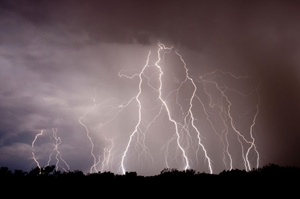
\includegraphics[scale=1.3]{DSC-B0818_09.jpg}
\caption{A.T. Willett/Alamy Stock Photo}
\end{figure}

\item \textbf{The stock market} --  is itself a fractal, with occasional huge crashes or bubbles, and far more frequent smaller rises and falls.
\begin{figure}[H]
\centering
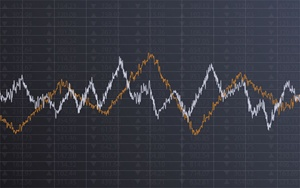
\includegraphics[scale=1.3]{DSC-B0818_10.jpg}
\caption{Champ008/Shutterstock}
\end{figure}

\item \textbf{DNA} -- is packed into a cell using a fractal pattern. The DNA in a human cell is 6.5 feet long — longer than the average human. But it has to be folded up to fit inside a tiny cell nucleus, and the cell must be able to unfold any bit of it that might be needed. A fractal pattern does the trick.
\begin{figure}[H]
\centering
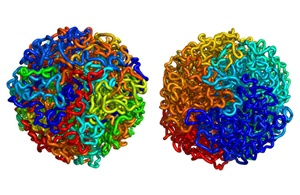
\includegraphics[scale=1.3]{DSC-B0818_11.jpg}
\caption{Leonid A. Mirny and Maxim Imakaev}
\end{figure}

\item \textbf{Ferns} -- provide another fractal example. Mathematician Michael Barnsley created a fern-shaped mathematical fractal (right) that could be mistaken for the real thing.
\begin{figure}[H]
\centering

\includegraphics[scale=1.3]{DSC-B0818_08.jpg}
\caption{Claudio Divizia/Shutterstock}
\end{figure}

\item \textbf{Clouds} --  form fractals, likely because wind turbulence operates similarly at a variety of scales. Large flows of warm, moist air rise in thermals, but within those are smaller columns of air twisting in their own shapes. So large- and small-scale formations end up looking alike.
\begin{figure}[H]
\centering
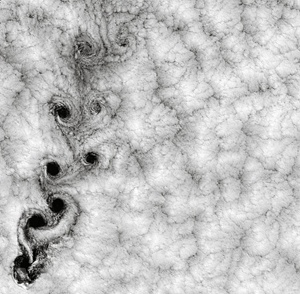
\includegraphics[scale=1.3]{DSC-B0818_12.jpg}
\caption{GSFC/NASA}
\end{figure}

\item \textbf{Human breast tissue} --  has a fractal structure, with the cells aligning into squiggles with squiggles in their squiggles. A pair of researchers at the University of Alberta analyzed nearly 8,000 images of healthy and cancerous tissues, and found that the fractal dimension of the cancerous tissue was consistently lower.
\begin{figure}[H]
\centering
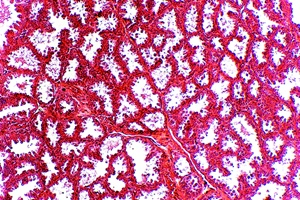
\includegraphics[scale=1.1]{DSC-B0818_13.jpg}
\caption{Keith Wheeler/Science Source}
\end{figure}
\section{Putting Fractals to Work}
It’s not only nature that loves fractals. Human beings have picked up on nature’s tricks, making use of fractals in our own technology.
\begin{figure}[H]
\centering
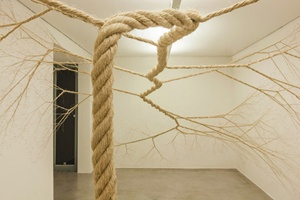
\includegraphics[scale=1.3]{DSC-B0818_14.jpg}
\caption{Ciclotrama 20 ( wind) rope sculpture by Janaina Mello Landini, photograph by Gui Gomes}
\end{figure}

\textbf{Ropes:} One of the earliest examples of using fractals to solve a problem involves ropes, as demonstrated in this sculpture by Janaina Mello Landini, titled Ciclotrama 20. Fine fibers are wound together into threads; threads are wound together into cords; cords are wound into cables.
\begin{figure}[H]
\centering
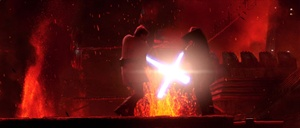
\includegraphics[scale=1.3]{DSC-B0818_15.jpg}
\caption{Animation}
\end{figure}

\textbf{Animation:} Since nature uses fractals, animators can exploit the blueprint to create good imitations. Animated films use fractals to create waves, snow or landscapes. The technique created a realistic simulation of lava in Star Wars: Episode III — Revenge of the Sith. 

\textbf{Fractal antennas:} The different scales of a fractal can be used to pick up different ranges of wavelengths of a signal, allowing a more powerful antenna in a small space.
\begin{figure}[H]
\centering
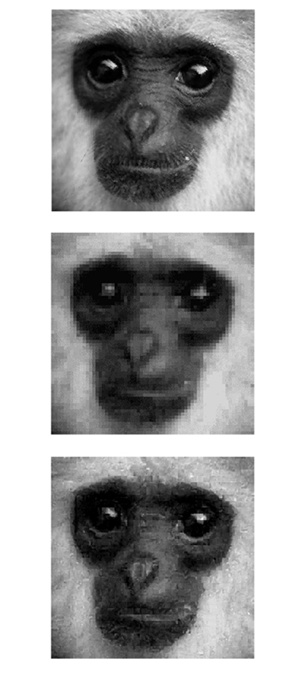
\includegraphics[scale=0.45]{DSC-B0818_18.jpg}
\caption{Compression}
\end{figure}

\textbf{Fractal compression:} Because high-quality photographs require so much data, we often use “compressed” versions that aren’t quite perfect, but are close. One such method looks for repeated patterns at different scales of a picture. It typically generates higher-quality images than the industry standard, a JPEG file, but isn’t common because it requires extra processing time.

\section{Mandelbrot Magic}
Below you can see the fractal generated by iterating the equation:
\Large $$Z_{n+1} = Z_{n} \cdot sin(Z_{n})$$ \normalsize
On the left is the big view of the fractal image, and on the right is a zoomed in detail, showing one of the infinite number of Mandelbrot replicas in this fractal.
\begin{figure}[H]
\centering
\hbox{\hspace{2em}
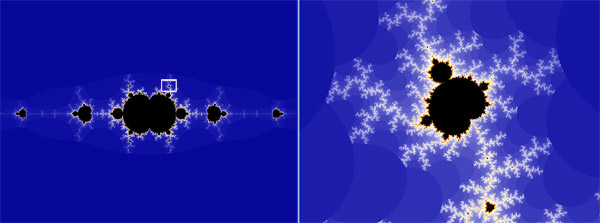
\includegraphics[scale=0.55]{sinusoidal.jpg}}
\caption{Sinusoidal fractal}
\end{figure}
Let's look at another example. This next fractal has been called the 'Nova' fractal, and it is generated by iterating the equation:
\Large $$Z_{n+1} = Z_{n} - \frac{(Z_{n}-1)^3}{(3 \cdot Z_{n}^2)} + C$$ \normalsize
On the left is the big view of the Nova fractal, and on the right is a zoomed-in detail, showing a perfect Mandelbrot replica.
\begin{figure}[H]
\centering
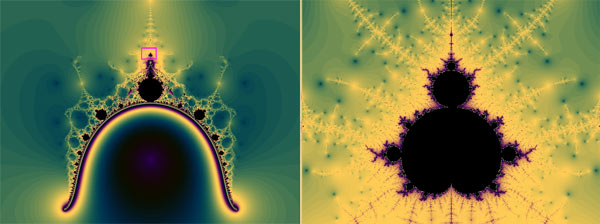
\includegraphics[scale=0.55]{nova.jpg}
\caption{Nova fractal}
\end{figure}
Finally, let's examine the "Magnet" fractal, which is particularly interesting, because it comes from an equation in physics that describes the way in which metals such as iron can gain or lose their magnetism. The equation is:
\Large $$Z_{n+1} = \sqrt \frac{Z_{n}^2 + C - 1}{2 \cdot Z_{n} + C -2}$$ \normalsize
\begin{figure}[H]
\centering
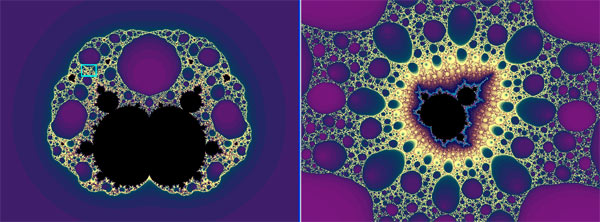
\includegraphics[scale=0.55]{magnet.jpg}
\caption{Magnet fractal}
\end{figure}


\end{itemize}
\newpage
\tableofcontents
\listoftables
\listoffigures
\begin{thebibliography}{9}
\bibitem{Urban}
 Yanguang Chen,
 \emph{How to Understand Fractals and Fractal Dimension
 of Urban Morphology}.
 Department of Geography, College of Urban and Environmental        Sciences, Peking University, Beijing
 2018.
 \bibitem{Chaos}
 Paul S. Addison,
 \emph{Fractals and Chaos: An Illustrated Course.}
 Institute of Physics Publishing, Bristol.
 1997.
 \bibitem{Mandelbrot}
 https://fractalfoundation.org/OFC/OFC-5-5.html
 \bibitem{Beauty}
 Edyta Patrzalek,
 \emph{Fractals: Useful Beauty
(General Introduction to Fractal Geometry)}.
 Stan Ackermans Institute,
 IPO, Centre for User-System Interaction, Eindhoven  University of Technology
 \bibitem{Lewis}
 Lewis R.,
 \emph{Fractals In Your Future.}
  Ontario 2000.
  \bibitem{Turner}
 Turner, M.J.,
 \emph{Modeling Nature With Fractals.}
 Leicester 2000

\end{thebibliography}
\end{document}

